\documentclass[12pt]{article}
\usepackage{amsmath,amssymb}
\setlength{\oddsidemargin}{0in}
\setlength{\evensidemargin}{0in}
\setlength{\textheight}{9in}
\setlength{\textwidth}{6.5in}
\setlength{\topmargin}{-0.5in}
\usepackage{enumitem}
\usepackage[table]{xcolor}
\usepackage{graphicx}
\usepackage{listings}
\usepackage{float}
\usepackage{caption}
\usepackage{subcaption}
\newcommand{\Adv}{{\mathbf{Adv}}}       
\newcommand{\prp}{{\mathrm{prp}}}             
\newcommand{\calK}{{\cal K}}
\newcommand{\outputs}{{\Rightarrow}}                



% Use \textbf{Solution:}\\ to begin your solution.

%%%%%%%%%%%%%%%%%%%%%%%%%%%%%%%%%%%%%%%%%%%%%%%%%%%%%%%%%%%%%%%%%%%%%%%%%%%
\title{\bf Math 151A: Problem Set 6}
\date{ }
\author{\bf Prof. Schaeffer}

\begin{document}
\maketitle


{\small \textbf{Instructions}:
\begin{itemize}
\item Due on Tuesday, May 30th by 5pm.
\item Late HW will not be accepted.
\item Write down all of the details and attach your code to the end of the assignment for full credit (as a PDF).  
\item If you LaTeX your solutions, you will get $5\%$ extra credit. 
\item (T) are ``pencil-and-paper'' problems and (C) means that the problem includes a computational/programming component. 
\end{itemize}}

%Add \newpage  between problems if you are using this to LaTex your solutions
\vspace{1em}

%%%%%%%%%%%%%%%%%%%%%%%%%%%%%%%%%%%%%%%%%%%%%%%%%%%%%%%%
\begin{enumerate}[label=\bfseries Problem \arabic*:]






 
%%%%%%%%%%%%%%%%%%%%%%%%%%%%%%%%%%%%%%%%%%%%%
\item \textbf{(T) Quadrature}\\
Let $h=\frac{b-a}{3}$, $x_0=a$, $x_1=a+h$, and $x_2=b$. Find the degree of precision of the quadrature formula:
\begin{align*}
\int_a^b f(x) \, \text{dx}\approx \frac{9h}{4} f(x_1)+\frac{3h}{4} f(x_2)
\end{align*}
You can check your work with symbolic software, but to receive full credit you must show your work.



\vspace{1em}
\textbf{Solution:}\\
For $f(x)$ of degree $0$
\begin{align*}
    \int_a^b f(x) \, \text{dx}=x|_{a}^{b}=b-a
\end{align*}
and
\begin{align*}
    \frac{9h}{4} f(x_1)+\frac{3h}{4} f(x_2)=\frac{9(b-a)}{4\cdot 3}\cdot1+\frac{3(b-a)}{4\cdot 3}\cdot 1=\frac{3(b-a)}{4}+\frac{b-a}{4}=b-a
\end{align*}
, so $f(x)$ is exact for degree $0$.\\

For $f(x)$ of degree $1$
\begin{align*}
    \int_a^b f(x) \, \text{dx}=\frac{1}{2}x^2|_{a}^{b}=\frac{b^2-a^2}{2}
\end{align*}
and
\begin{multline*}
    \frac{9h}{4} f(x_1)+\frac{3h}{4} f(x_2)=\frac{9(b-a)}{4\cdot 3}\cdot (a+\frac{b-a}{3})+\frac{3(b-a)}{4\cdot 3}\cdot b=\frac{(b-a)(b+2a)}{4}+\frac{b(b-a)}{4}\\
    =\frac{(b-a)(2b+2a)}{4}=\frac{b^2-a^2}{2}
\end{multline*}
, so $f(x)$ is exact for degree $1$.\\

For $f(x)$ of degree $2$
\begin{align*}
    \int_a^b f(x) \, \text{dx}=\frac{1}{3}x^3|_{a}^{b}=\frac{b^3-a^3}{3}
\end{align*}
and
\begin{multline*}
    \frac{9h}{4} f(x_1)+\frac{3h}{4} f(x_2)=\frac{3(b-a)}{4}\cdot (\frac{b+2a}{3})^2+\frac{b-a}{4}\cdot b^2=\frac{(b-a)(b+2a)^2}{12}+\frac{b^2(b-a)}{4}\\
    =\frac{(b-a)(4b^2+4ab+4a^2)}{12}=\frac{b^3-a^3}{3}
\end{multline*}
, so $f(x)$ is exact for degree $2$.\\

For $f(x)$ of degree $3$
\begin{align*}
    \int_a^b f(x) \, \text{dx}=\frac{1}{4}x^4|_{a}^{b}=\frac{b^4-a^4}{4}
\end{align*}
and
\begin{multline*}
    \frac{9h}{4} f(x_1)+\frac{3h}{4} f(x_2)=\frac{3(b-a)}{4}\cdot (\frac{b+2a}{3})^3+\frac{b-a}{4}\cdot b^3=\frac{(b-a)(b+2a)^3}{36}+\frac{b^3(b-a)}{4}\\
    =\frac{(b-a)(10b^3+6ab^2+12a^2b+8a^3)}{36}=\frac{10b^4-4ab^3+6a^2b^2-4a^3b-8a^4}{36}\neq\frac{b^4-a^4}{4}
\end{multline*}
, so $f(x)$ is not exact for degree $3$.\\

Thus, the quadrature formula has degree of precision $2$.



\newpage 

 %%%%%%%%%%%%%%%%%%%%%%%%%%%%%%
 \item \textbf{(T) More Quadrature}\\
 Find the constants $a$, $x_0$, and $x_1$ so that the quadrature formula:
$$\int_0^1 f(x)\, \text{dx}\approx \frac{1}{2} f(x_0) + a f(x_1) $$
has the highest possible degree of precision.


\vspace{1em}
\textbf{Solution:}\\
For $f(x)$ of degree $0$
\begin{align*}
    \int_0^1 f(x) \, \text{dx}=x|_{0}^{1}=1
\end{align*}
and
\begin{align*}
    \frac{1}{2} f(x_0) + a f(x_1) =\frac{1}{2}+a
\end{align*}
, so $f(x)$ is exact for degree $0$ if $a=\frac{1}{2}$.\\

For $f(x)$ of degree $1$
\begin{align*}
    \int_0^1 f(x) \, \text{dx}=\frac{1}{2}x^2|_{0}^{1}=\frac{1}{2}
\end{align*}
and
\begin{align*}
    \frac{1}{2} f(x_0) + a f(x_1) = \frac{1}{2}x_0 + \frac{1}{2}x_1
\end{align*}
, so $f(x)$ is exact for degree $1$ if $a=\frac{1}{2}$ and $x_0+x_1=1$.\\

For $f(x)$ of degree $2$
\begin{align*}
    \int_0^1 f(x) \, \text{dx}=\frac{1}{3}x^3|_{0}^{1}=\frac{1}{3}
\end{align*}
and
\begin{align*}
    \frac{1}{2} f(x_0) + a f(x_1) = \frac{1}{2}x_0^2 + \frac{1}{2}(1-x_0)^2 = \frac{1}{2}-x_0+x_0^2
\end{align*}
, so $f(x)$ is exact for degree $2$ if $a=\frac{1}{2}$, $x_0=\frac{3-\sqrt{3}}{6}$, and $x_1=\frac{3+\sqrt{3}}{6}$.\\

For $f(x)$ of degree $3$
\begin{align*}
    \int_0^1 f(x) \, \text{dx}=\frac{1}{4}x^4|_{0}^{1}=\frac{1}{4}
\end{align*}
and
\begin{align*}
    \frac{1}{2} f(x_0) + a f(x_1) = \frac{1}{2}(\frac{3-\sqrt{3}}{6})^3 + \frac{1}{2}(\frac{3+\sqrt{3}}{6})^3 = \frac{1}{4} \textit{(plugged into a calculator)}
\end{align*}
, so $f(x)$ is exact for degree $3$ if $a=\frac{1}{2}$, $x_0=\frac{3-\sqrt{3}}{6}$, and $x_1=\frac{3+\sqrt{3}}{6}$.\\

For $f(x)$ of degree $4$
\begin{align*}
    \int_0^1 f(x) \, \text{dx}=\frac{1}{5}x^5|_{0}^{1}=\frac{1}{5}
\end{align*}
and
\begin{align*}
    \frac{1}{2} f(x_0) + a f(x_1) = \frac{1}{2}(\frac{3-\sqrt{3}}{6})^4 + \frac{1}{2}(\frac{3+\sqrt{3}}{6})^4 = 0.19\overline{4} \textit{(plugged into a calculator)}
\end{align*}
, so $f(x)$ is not exact for degree $4$ for any such combination of $a,x_0,$ and $x_1$ that is also exact for polynomials of degree-3 or less.\\

Thus, $$\int_0^1 f(x)\, \text{dx}\approx \frac{1}{2} f(x_0) + a f(x_1) $$ can have precision of at most degree-3 with coefficients $a=\frac{1}{2}$, $x_0=\frac{3-\sqrt{3}}{6},$ and $x_1=\frac{3+\sqrt{3}}{6}$
\newpage 

%%%%%%%%%%%%%%%%%%%%%%%%%%%%%%
 \item \textbf{(T) Even More Quadrature}\\
Determine the constants $a$, $b$, $c$, and $d$ that will produce a quadrature formula:
$$\int_{-1}^1 f(x) \,\text{dx} \approx a f(-1) + b f(1)+ c f'(-1)+ d f'(1) $$
that is exact to degree three.



\vspace{1em}
\textbf{Solution:}\\
For $f(x)$ of degree $0$
\begin{align*}
    \int_{-1}^1 f(x) \, \text{dx}=x|_{-1}^{1}=2
\end{align*}
and
\begin{align*}
    a f(-1) + b f(1)+ c f'(-1)+ d f'(1)=a\cdot1+b\cdot1
\end{align*}
, so $f(x)$ is exact for degree $0$ if $a+b=2$.\\

For $f(x)$ of degree $1$
\begin{align*}
    \int_{-1}^1 f(x) \, \text{dx}=\frac{1}{2}x^2|_{-1}^{1}=0
\end{align*}
and
\begin{align*}
    a f(-1) + b f(1)+ c f'(-1)+ d f'(1)=-a + b + c + d
\end{align*}
, so $f(x)$ is exact for degree $1$ if $a+b=2$ and $-a+b+c+d=0$.\\

For $f(x)$ of degree $2$
\begin{align*}
    \int_{-1}^1 f(x) \, \text{dx}=\frac{1}{3}x^3|_{-1}^{1}=\frac{2}{3}
\end{align*}
and
\begin{align*}
    a f(-1) + b f(1)+ c f'(-1)+ d f'(1)=a(-1)^2 + b(1)^2 + c(2\cdot(-1)) + d(2\cdot(1)) = a + b - 2c + 2d
\end{align*}
, so $f(x)$ is exact for degree $2$ if $a+b=2$, $-a+b+c+d=0$, and $a+b-2c+2d=\frac{2}{3}$.\\

For $f(x)$ of degree $3$
\begin{align*}
    \int_{-1}^1 f(x) \, \text{dx}=\frac{1}{4}x^4|_{-1}^{1}=0
\end{align*}
and
\begin{multline*}
    a f(-1) + b f(1)+ c f'(-1)+ d f'(1)\\
    =a(-1)^3 + b(1)^3 + c(3(1)^2) + d(3(-1)^2) = -a+b+3c+3d
\end{multline*}
, so $f(x)$ is exact for degree $2$ if\\ $a+b=2$, $-a+b+c+d=0$, $a+b-2c+2d=\frac{2}{3}$, and $-a+b+3c+3d=0$.\\

$\begin{bmatrix}
    1 & 1 & 0 & 0\\
    -1 & 1 & 1 & 1\\
    1 & 1 & -2 & 2\\
    -1 & 1 & 3 & 3\\
\end{bmatrix}
\times
\begin{bmatrix}
    a\\
    b\\
    c\\
    d\\
\end{bmatrix}
=
\begin{bmatrix}
    2\\
    0\\
    \frac{2}{3}\\
    0\\
\end{bmatrix}
$


Thus, 
$$\int_{-1}^1 f(x) \,\text{dx} \approx 1 f(-1) + 1 f(1) + \frac{1}{3} f'(-1) - \frac{1}{3} f'(1) $$
 is exact to degree three.
\newpage 

%%%%%%%%%%%%%%%%%%%%%%%%%%%%%%
 \item \textbf{(C) Edge Detector}\\
Complete the template code ``MyEdgeDetector.m'' by filling in the missing lines. You will need to choose a finite difference method (either forward, backward, or central), and tune the parameters (`thres' and the parameters in `G' on line 25).  The two example images provided are `3.gif' and `cameraman.png' from class. You will need to include a third example of your choosing (see line 15). You will need to submit \textbf{four images}: the edge maps for the two examples provided, the original grayscale image for your third example, and the edge map for the third example. Attach your code for full credit. 

\vspace{1em}
\textbf{Solution:}\\
    \begin{figure}[H]
        \begin{subfigure}[t!]{.5\textwidth}
            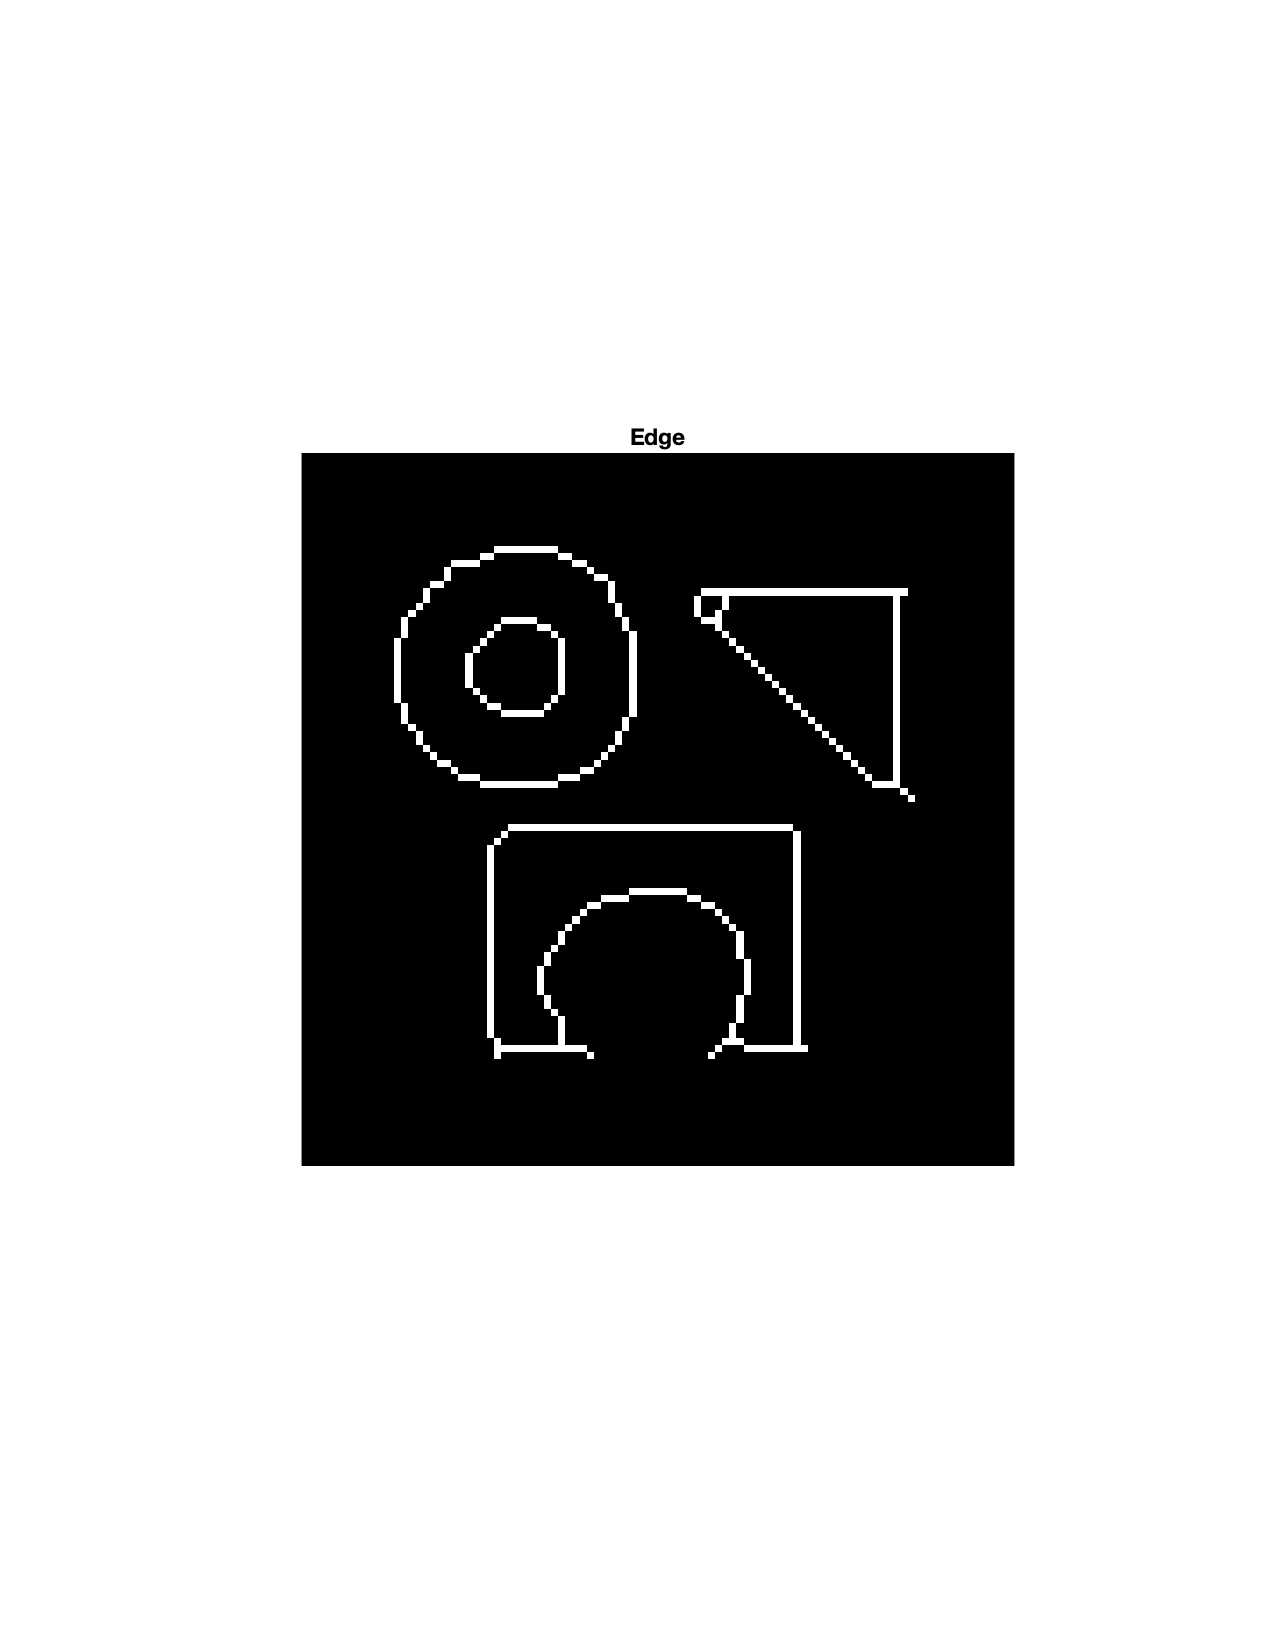
\includegraphics[width=\linewidth]{MyEdgeDetector_1.pdf}
        \end{subfigure}%
        \begin{subfigure}[t!]{.5\textwidth}
            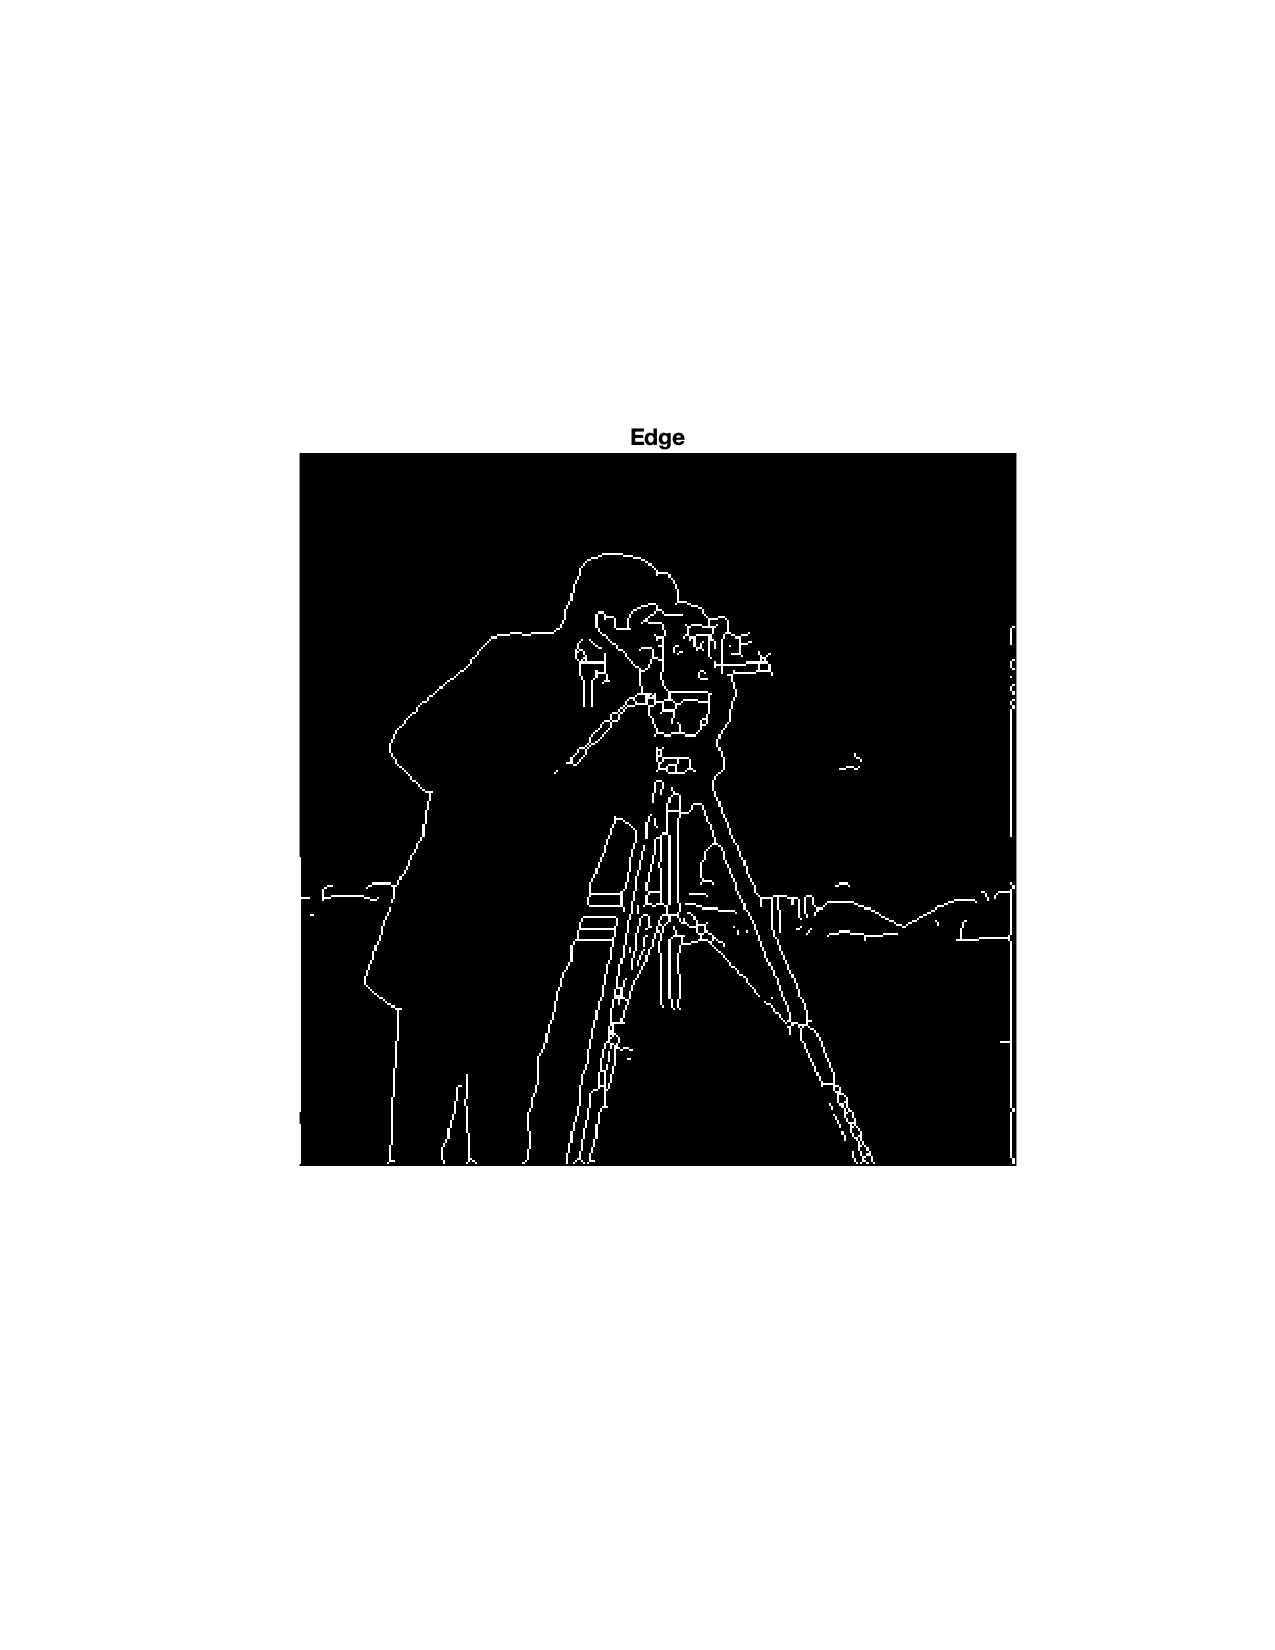
\includegraphics[width=\linewidth]{MyEdgeDetector_2.pdf}
        \end{subfigure}%
    \end{figure} 
    \begin{figure}[H]
        \begin{subfigure}[t!]{.5\textwidth}
            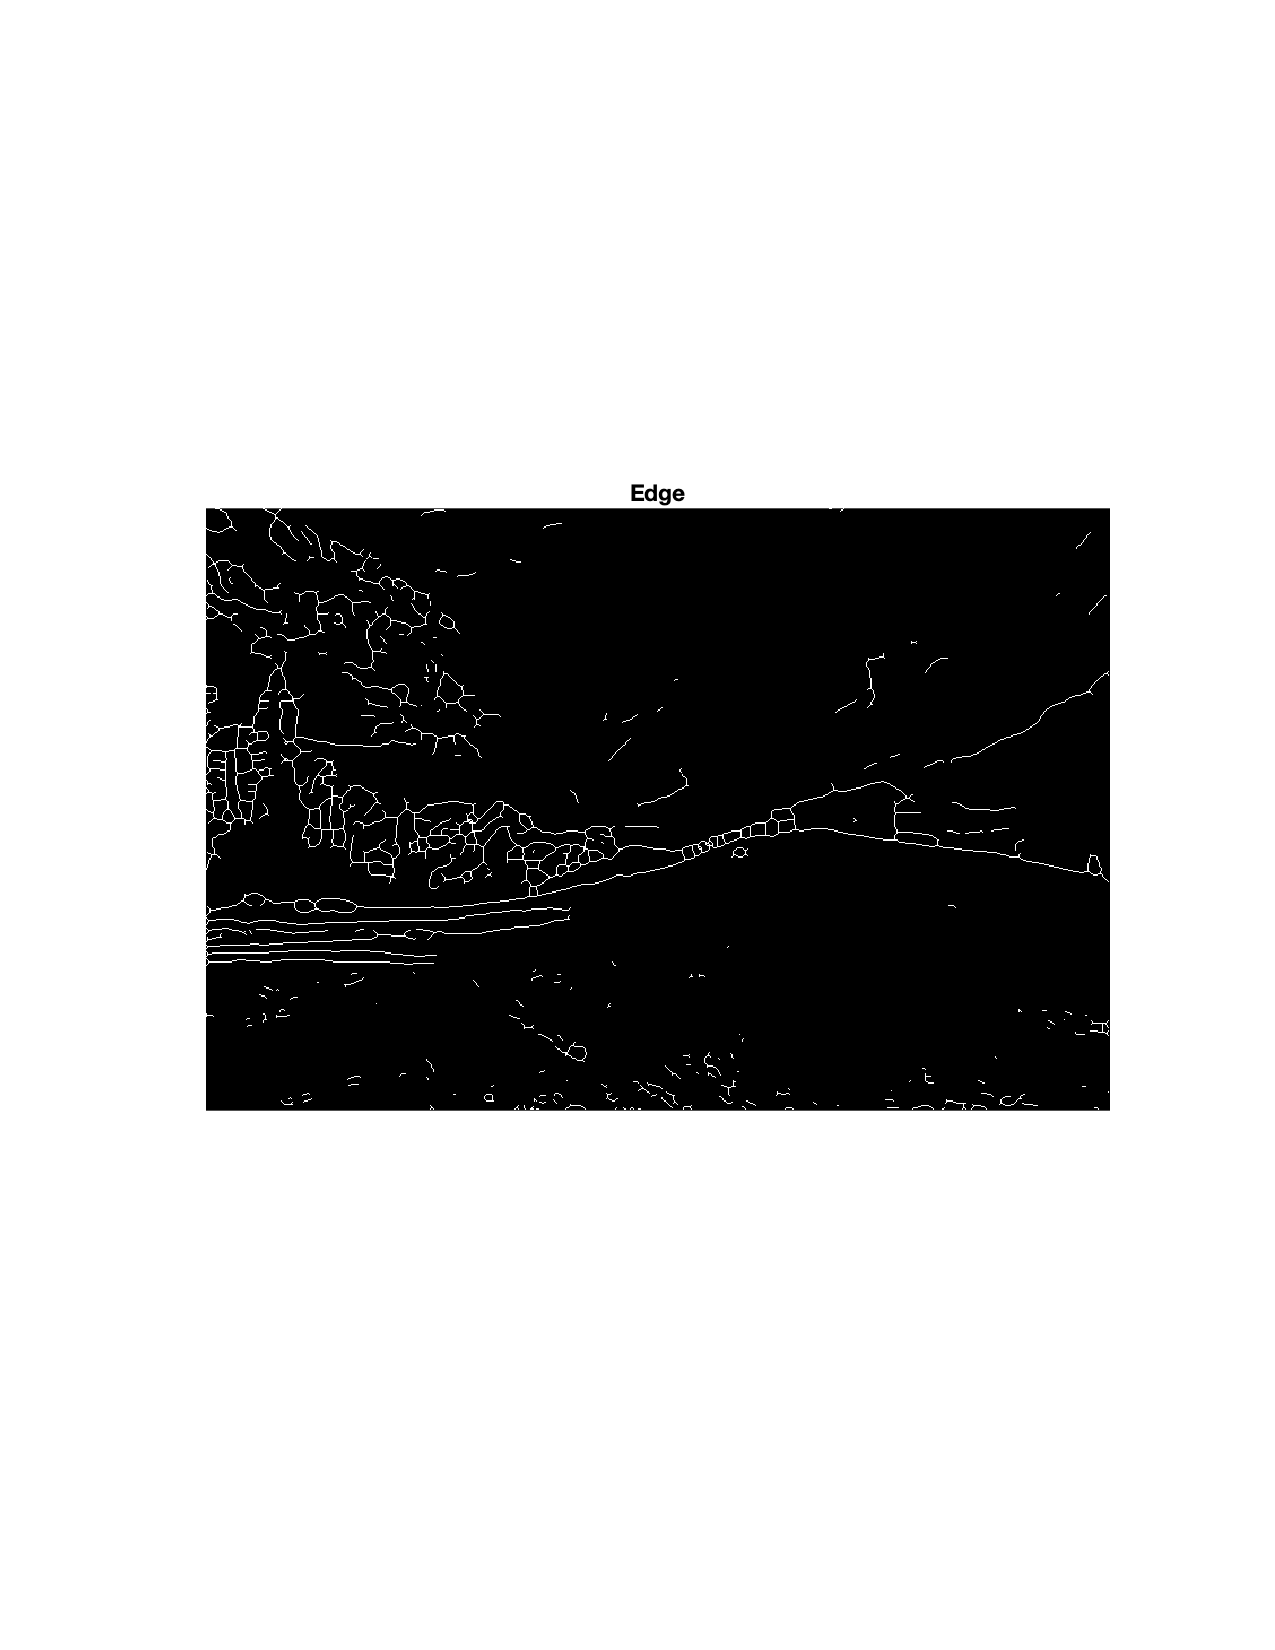
\includegraphics[width=\linewidth]{MyEdgeDetector_3.pdf}
        \end{subfigure}%
        \begin{subfigure}[t!]{.5\textwidth}
            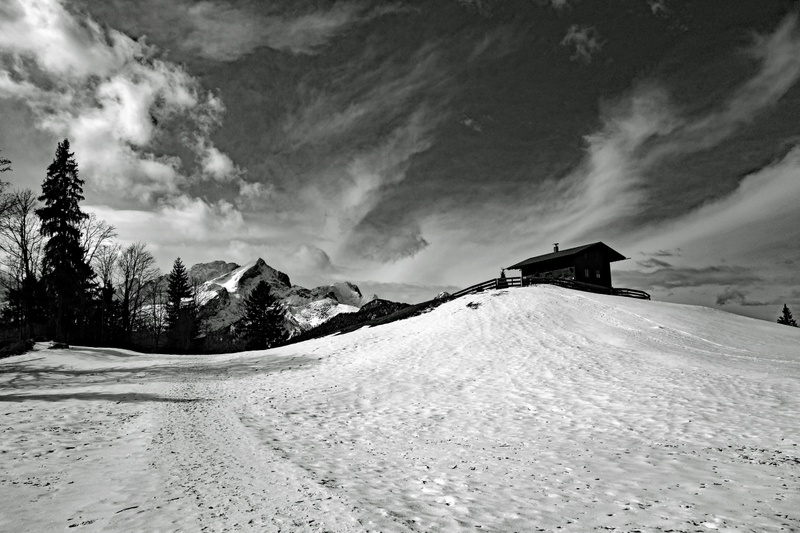
\includegraphics[width=\linewidth]{winter-landscape.jpg}
        \end{subfigure}%
    \end{figure}
    \begin{figure}
        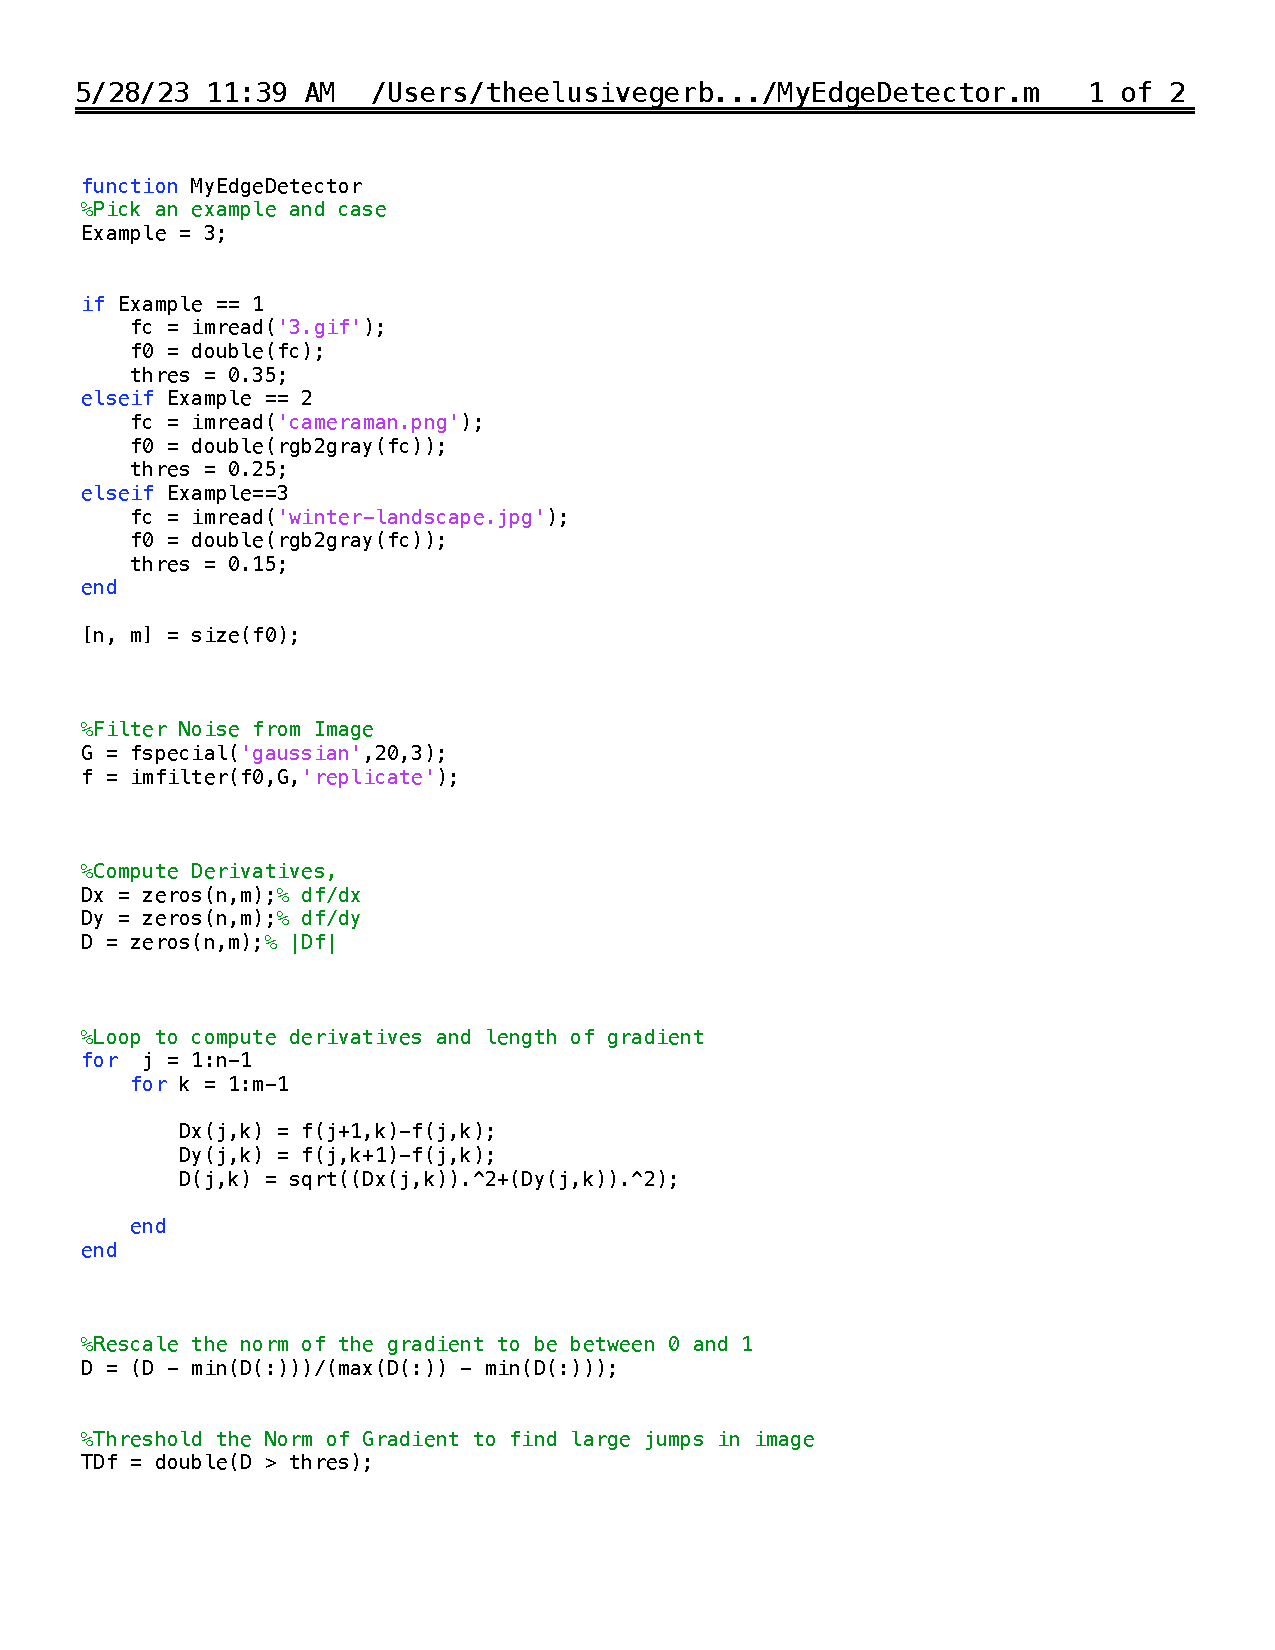
\includegraphics[width=\linewidth]{MyEdgeDetector_code.pdf}
    \end{figure}    
%%%%%%%%%%%%%%%%%%%%%%%%%%%%%%%%%%%





\end{enumerate}

\end{document}


